\chapter{\LaTeX\ Tips and Tricks}\label{chap:tipstricks}

In this chapter, we show some useful tips and tricks when working with \LaTeX.

\section{Using Git}

We recommend you to use \emph{Git} also for your \LaTeX\ files such as this report.
If you do so, we suggest to write every sentence in your \TeX\ file on a new line.
This will make it easier to keep track of changes since \emph{Git} tracks them line by line.
So if you change one sentence, \emph{Git} will tell you that only that sentence has changed instead of the entire paragraph otherwise.
Furthermore, if you are using the PDF viewer of \emph{texmaker}, you can jump from the PDF directly to the sentence in the \TeX\ file by clicking on it (instead of just jumping to the corresponding paragraph).

\section{Headings}

Your report can be structured using several different types of headings.
Use the commands \textbackslash\texttt{chapter}\{.\}, \textbackslash\texttt{section}\{.\}, \textbackslash\texttt{subsection}\{.\}, and \textbackslash\texttt{subsubsection}\{.\}.
Use the asterisk symbol \texttt{*} to suppress numbering of a certain heading if necessary, for example, \textbackslash\texttt{section*}\{.\}.


\section{References}\label{sec:references}

References to literature are included using the command \textbackslash\texttt{cite}\{$\cdot$\}.
For example \cite{KleinMurray2007,Strasdat2010WhyFilter}.
Your references must be entered in the file \texttt{bibliography.bib}.
Making changes or adding new references in the bibliography file can be done manually or by using specialized software such as \textit{JabRef} which is free of charge.

Cross-referencing within the text is easily done using \textbackslash\texttt{label}\{$\cdot$\} and \textbackslash\texttt{ref}\{$\cdot$\}.
For example, this paragraph is part of Chapter~\ref{chap:tipstricks}; more specifically on page~\pageref{sec:references}.

\section{Writing Equations}\label{sec:math}

The most common way to include equations is using the \texttt{equation} environment.
Use \textbackslash\texttt{eqref}\{$\cdot$\} to reference an equation, e.g., \eqref{eq:pose_candidates}.

Embed equations in the text.
Thus you must use proper punctuation.
You must introduce all symbols that you use.
You should define these before you use them.
However, they must be introduced in the same sentence at the latest. 

\subsection*{Example 1}

For $n$ detections and $m$ LEDs on the object, we will
obtain $N$ pose candidates,
% (this is to avoid extra space)
	\begin{equation}\label{eq:pose_candidates}
		N =  4 \alpha \binom{n}{3} \frac{m!}{(m-3)!},
	\end{equation}
% (this is to avoid extra space)
where $\alpha \in \left\{ {1, 2}\right\}$ is a magic factor.

\subsection*{Example 2}

The transformation matrix in homogeneous coordinates, $\mathtt{T}$, is composed of the rotation matrix $\mathbf{R}$ and translation vector $\mathbf{p}$,
% (this is to avoid extra space)
  \begin{equation}\label{eq:se3}
    \mathtt{T} = \begin{bmatrix}\mathbf{R} & \mathbf{p} \\ 0 & 1\end{bmatrix}, \qquad \text{with} \quad \mathbf{R} \in SO(3), \ \ \mathbf{p} \in \mathbb{R}^3.
  \end{equation}


\section{Including Graphics}\label{sec:epsgraph}

The easiest way to include figures in your document is to use PDF figures if you use \texttt{pdflatex} to compile.
Figure \ref{img:notation} was created with the use of the open-source program \texttt{ipe}.

  \begin{figure}[h]
     \centering
     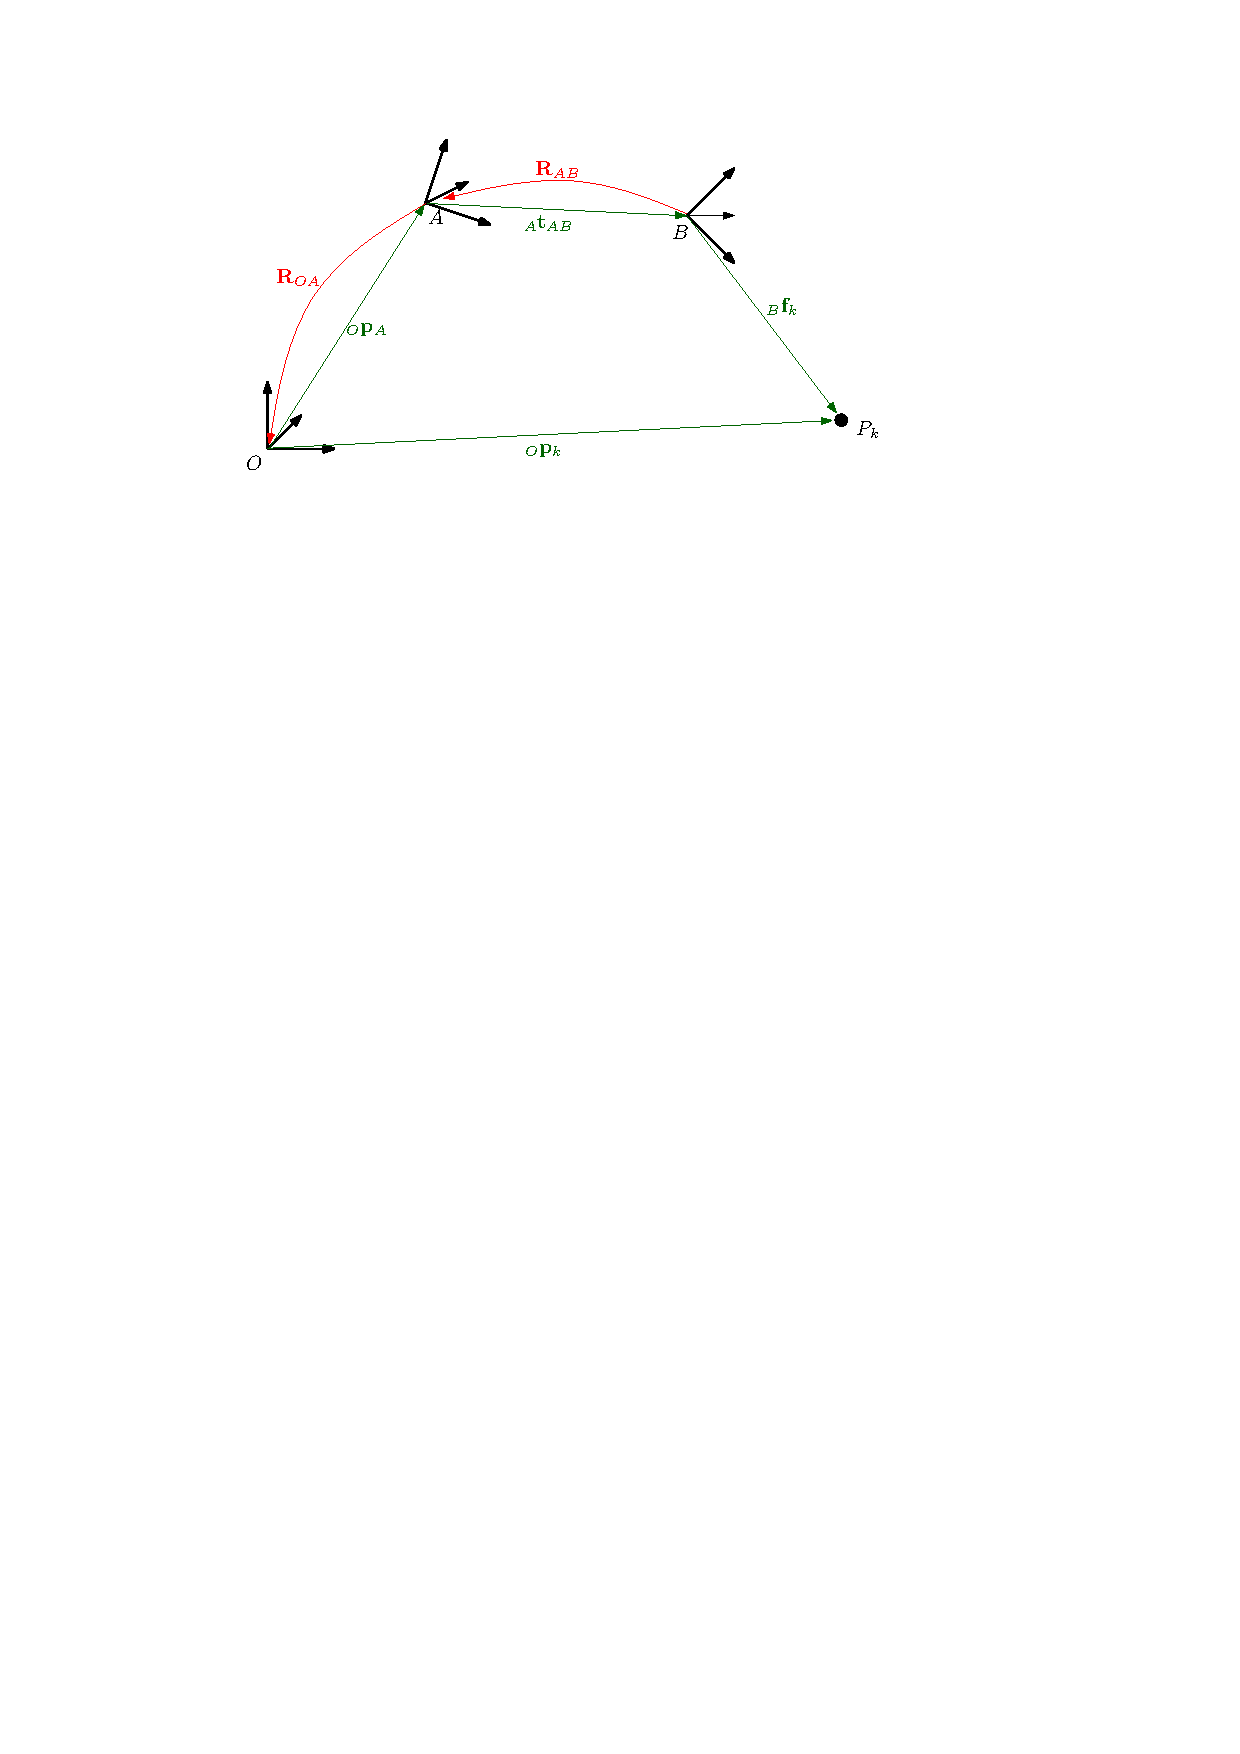
\includegraphics[width=0.6\textwidth]{img/notation.pdf}
     \caption{Example of a figure.}
     \label{img:notation}
  \end{figure}

\section{Including Matlab Figures}

When including figures into your report you want them as a vector graphic such that you can zoom into the figure without getting blurry.
Furthermore it is nice when the text in the figure gets substituted by \LaTeX\ such that you have the same font and the same font size.
Figure \ref{fig:example_tikz_figure} shows an example of such an imported matlab figure.
An easy way of achieving this is by using the \texttt{matlab2tikz} script.
You can find a short example on how to use this script in the \texttt{matlab\_figures} folder.
The \texttt{create\_figures.m} script creates a plot and then the tikz file which you can include in your document.
For using tikz, you need to make use of the \texttt{pgfplots} package in your \TeX\ document.
More information on using \texttt{matlab2tikz} can be found on \href{http://www.mathworks.com/matlabcentral/fileexchange/22022-matlab2tikz}{Matlab Central} where you can also download the necessary files (\texttt{matlab2tikz.m}, \texttt{matlab2tikzInputParser.m}, \texttt{updater.m}).

\begin{figure}[H]
  \centering
  \setlength\fwidth{8.0cm}
  \setlength\fheight{6.0cm}
  % This file was created by matlab2tikz v0.4.7 running on MATLAB 8.0.
% Copyright (c) 2008--2014, Nico Schlömer <nico.schloemer@gmail.com>
% All rights reserved.
% Minimal pgfplots version: 1.3
% 
% The latest updates can be retrieved from
%   http://www.mathworks.com/matlabcentral/fileexchange/22022-matlab2tikz
% where you can also make suggestions and rate matlab2tikz.
% 
\begin{tikzpicture}

\begin{axis}[%
width=\fwidth,
height=\fheight,
scale only axis,
xmin=0,
xmax=10,
xlabel={time [$s$]},
ymin=-1,
ymax=1,
ylabel={velocity [$\frac{m}{s}$]},
legend style={draw=black,fill=white,legend cell align=left}
]
\addplot [color=blue,solid]
  table[row sep=crcr]{0	0\\
0.101010101010101	0.100838420258105\\
0.202020202020202	0.200648856522685\\
0.303030303030303	0.298413804447641\\
0.404040404040404	0.39313661214833\\
0.505050505050505	0.483851640437935\\
0.606060606060606	0.569634106908966\\
0.707070707070707	0.649609513505707\\
0.808080808080808	0.72296256147946\\
0.909090909090909	0.788945462844257\\
1.01010101010101	0.846885563602983\\
1.11111111111111	0.896192201029956\\
1.21212121212121	0.936362725104285\\
1.31313131313131	0.9669876227093\\
1.41414141414141	0.987754692360084\\
1.51515151515152	0.998452226900389\\
1.61616161616162	0.998971171723357\\
1.71717171717172	0.98930623651434\\
1.81818181818182	0.969555949182324\\
1.91919191919192	0.939921651430131\\
2.02020202020202	0.900705446202955\\
2.12121212121212	0.852307117939675\\
2.22222222222222	0.795220057023049\\
2.32323232323232	0.730026229976446\\
2.42424242424242	0.657390246682775\\
2.52525252525253	0.578052585106573\\
2.62626262626263	0.492822042588923\\
2.72727272727273	0.402567490669497\\
2.82828282828283	0.308209017490077\\
2.92929292929293	0.210708548077192\\
3.03030303030303	0.11106003812413\\
3.13131313131313	0.0102793412405343\\
3.23232323232323	-0.0906061470334077\\
3.33333333333333	-0.190567962875485\\
3.43434343434343	-0.288587058720432\\
3.53535353535354	-0.383664191806112\\
3.63636363636364	-0.474830110822239\\
3.73737373737374	-0.561155436815202\\
3.83838383838384	-0.641760137619388\\
3.93939393939394	-0.71582249922919\\
4.04040404040404	-0.782587502654202\\
4.14141414141414	-0.84137452086087\\
4.24242424242424	-0.89158425733514\\
4.34343434343434	-0.932704855531834\\
4.44444444444444	-0.964317116928778\\
4.54545454545455	-0.98609877449093\\
4.64646464646465	-0.997827777979213\\
4.74747474747475	-0.999384557612436\\
4.84848484848485	-0.990753243005677\\
4.94949494949495	-0.972021824958833\\
5.05050505050505	-0.943381258446\\
5.15151515151515	-0.905123515950137\\
5.25252525252525	-0.857638610988052\\
5.35353535353535	-0.80141062216897\\
5.45454545454545	-0.737012758318913\\
5.55555555555556	-0.665101514978822\\
5.65656565656566	-0.586409981847235\\
5.75757575757576	-0.501740369393911\\
5.85858585858586	-0.411955830830862\\
5.95959595959596	-0.317971662810619\\
6.06060606060606	-0.220745974555063\\
6.16161616161616	-0.121269920537167\\
6.26262626262626	-0.0205575962872592\\
6.36363636363636	0.0803642996702817\\
6.46464646464646	0.180466932359911\\
6.56565656565657	0.278729818677557\\
6.66666666666667	0.37415123057122\\
6.76767676767677	0.465758407025652\\
6.86868686868687	0.552617470746406\\
6.96969696969697	0.633842948448906\\
7.07070707070707	0.708606797699218\\
7.17171717171717	0.776146848283581\\
7.27272727272727	0.835774572052259\\
7.37373737373737	0.886882102029079\\
7.47474747474747	0.928948429231251\\
7.57575757575758	0.961544714026824\\
7.67676767676768	0.984338657883824\\
7.77777777777778	0.997097890943875\\
7.87878787878788	0.999692340886112\\
7.97979797979798	0.992095558932323\\
8.08080808080808	0.974384989475536\\
8.18181818181818	0.946741180583354\\
8.28282828282828	0.909445943424462\\
8.38383838383838	0.862879479381784\\
8.48484848484848	0.807516504139563\\
8.58585858585859	0.743921408256844\\
8.68686868686869	0.672742503562265\\
8.78787878787879	0.594705414024498\\
8.88888888888889	0.510605678474283\\
8.98989898989899	0.421300640588607\\
9.09090909090909	0.327700708813498\\
9.19191919191919	0.230760075325052\\
9.29292929292929	0.131466988642958\\
9.39393939393939	0.030833679061141\\
9.49494949494949	-0.0701139604006468\\
9.5959595959596	-0.170346832328096\\
9.6969696969697	-0.268843125910384\\
9.7979797979798	-0.364598733655889\\
9.8989898989899	-0.456637487633774\\
10	-0.54402111088937\\
};
\addlegendentry{Robot a};

\addplot [color=red,solid]
  table[row sep=crcr]{0	1\\
0.101010101010101	0.99490281585683\\
0.202020202020202	0.9796632259997\\
0.303030303030303	0.954436588420145\\
0.404040404040404	0.919480072752278\\
0.505050505050505	0.875150038590823\\
0.606060606060606	0.82189840263017\\
0.707070707070707	0.760268031659151\\
0.808080808080808	0.690887208377067\\
0.909090909090909	0.614463226448467\\
1.01010101010101	0.531775180091039\\
1.11111111111111	0.443666021702229\\
1.21212121212121	0.35103396849205\\
1.31313131313131	0.254823345726049\\
1.41414141414141	0.156014959925759\\
1.51515151515152	0.0556161001658067\\
1.61616161616162	-0.0453497306018852\\
1.71717171717172	-0.145853249514135\\
1.81818181818182	-0.244869886685079\\
1.91919191919192	-0.341390230048921\\
2.02020202020202	-0.434430315678286\\
2.12121212121212	-0.523041658674875\\
2.22222222222222	-0.606320922373835\\
2.32323232323232	-0.683419127290403\\
2.42424242424242	-0.753550305929445\\
2.52525252525253	-0.815999515227557\\
2.62626262626263	-0.870130124945965\\
2.72727272727273	-0.915390307713636\\
2.82828282828283	-0.951318664558728\\
2.92929292929293	-0.97754892857964\\
3.03030303030303	-0.993813698804694\\
3.13131313131313	-0.999947166176124\\
3.23232323232323	-0.995886803868673\\
3.33333333333333	-0.981674004711079\\
3.43434343434343	-0.957453659212335\\
3.53535353535354	-0.923472678494476\\
3.63636363636364	-0.880077477189673\\
3.73737373737374	-0.827710441961886\\
3.83838383838384	-0.76690542165429\\
3.93939393939394	-0.69828228503756\\
4.04040404040404	-0.62254060163933\\
4.14141414141414	-0.54045251007479\\
4.24242424242424	-0.452854846581271\\
4.34343434343434	-0.360640614001448\\
4.44444444444444	-0.264749878183483\\
4.54545454545455	-0.166160184603552\\
4.64646464646465	-0.0658765929072468\\
4.74747474747475	0.0350785690386048\\
4.84848484848485	0.135676127132719\\
4.94949494949495	0.234890552819178\\
5.05050505050505	0.331710417703216\\
5.15151515151515	0.425148704424772\\
5.25252525252525	0.514252868676963\\
5.35353535353535	0.598114549793553\\
5.45454545454545	0.67587883091213\\
5.55555555555556	0.746752954311448\\
5.65656565656566	0.810014403075603\\
5.75757575757576	0.865018266697566\\
5.85858585858586	0.911203815534403\\
5.95959595959596	0.948100217091764\\
6.06060606060606	0.975331335863734\\
6.16161616161616	0.992619567796701\\
6.26262626262626	0.999788670287321\\
6.36363636363636	0.996765558864523\\
6.46464646464646	0.983581052239521\\
6.56565656565657	0.960369558128524\\
6.66666666666667	0.927367703050975\\
6.76767676767677	0.884911920071669\\
6.86868686868687	0.833435019078179\\
6.96969696969697	0.773461774557475\\
7.07070707070707	0.705603575851525\\
7.17171717171717	0.630552194429187\\
7.27272727272727	0.54907273171308\\
7.37373737373737	0.461995819353901\\
7.47474747474747	0.37020915146548\\
7.57575757575758	0.274648435144047\\
7.67676767676768	0.176287851525489\\
7.77777777777778	0.0761301246240719\\
7.87878787878788	-0.0248037008054478\\
7.97979797979798	-0.125484668174093\\
8.08080808080808	-0.224886398621082\\
8.18181818181818	-0.321995554297938\\
8.28282828282828	-0.415822168707717\\
8.38383838383838	-0.505409738788067\\
8.48484848484848	-0.589844975855707\\
8.58585858585859	-0.668267116007629\\
8.68686868686869	-0.739876695065317\\
8.78787878787879	-0.80394369860703\\
8.88888888888889	-0.859815004003662\\
8.98989898989899	-0.906921038591359\\
9.09090909090909	-0.944781586105027\\
9.19191919191919	-0.973010682179788\\
9.29292929292929	-0.991320549013866\\
9.39393939393939	-0.99952452908148\\
9.49494949494949	-0.997538987988408\\
9.5959595959596	-0.985384167071799\\
9.6969696969697	-0.963183977052532\\
9.7979797979798	-0.931164734843692\\
9.8989898989899	-0.889652856392602\\
10	-0.839071529076452\\
};
\addlegendentry{Robot b};

\end{axis}
\end{tikzpicture}%
  \caption{Example figure created with \texttt{matlab2tikz}.}
  \label{fig:example_tikz_figure}
\end{figure}

An alternative which you might want to consider is \texttt{matlabfrag} and \texttt{mlf2pdf}.
Especially when there are many data points in your figure you might run into problems when using tikz.
Again, you can find a short example on how to use \texttt{mlf2pdf} in the \texttt{create\_figures.m} scriptin in the \texttt{matlab\_figures} folder.
This script makes use of the two functions \texttt{matlabfrag.m} and \texttt{mlf2pdf.m} to create a PDF which you can then include into matlab.
These two files can be downloaded \href{http://www.mathworks.ch/matlabcentral/fileexchange/28545-matlabfrag-to-pdf}{here} and \href{http://www.mathworks.ch/matlabcentral/fileexchange/21286-matlabfrag}{here}.

\begin{figure}[H]
     \centering
     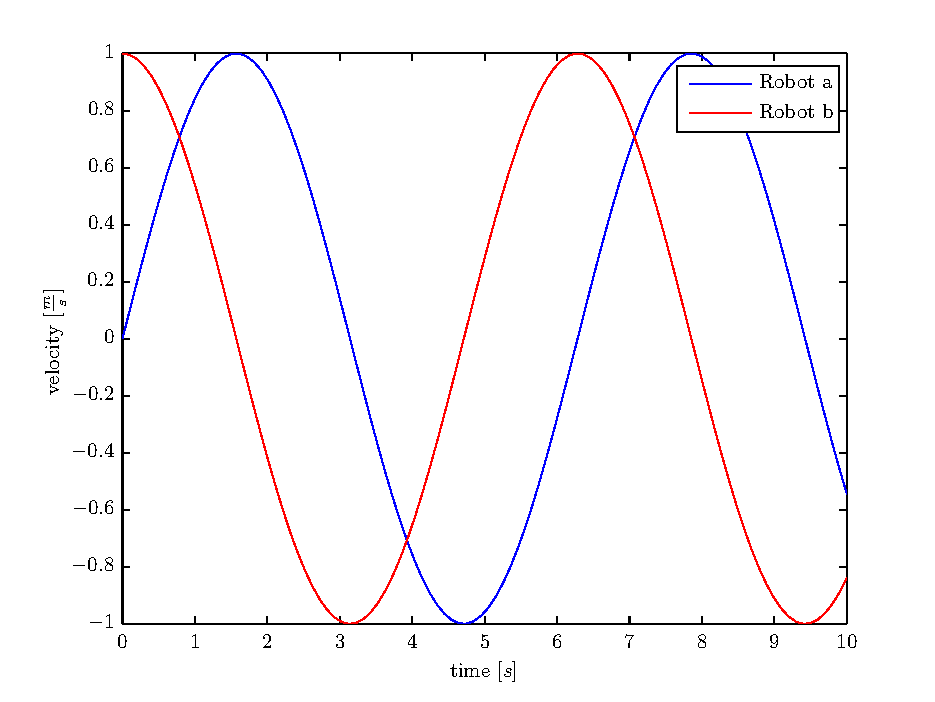
\includegraphics[width=0.85\textwidth]{matlab_figures/example_matlabfrag_figure.pdf}
     \caption{Example figure created with \texttt{mlf2pdf}.}
     \label{fig:example_matlab_fig}
  \end{figure}


\section{Including Code in your Document}

You may include samples from your Matlab code using the \texttt{lstlistings} environment, for example:

  \lstset{language=Matlab,numbers=none}
  \begin{lstlisting}[frame=lines, caption=Matlab Example, label=matlabexample]
  % Evaluate y = 2x
  for i = 1:length(x)

    y(i) = 2*x(i);

  end
  \end{lstlisting}

  \lstset{language=C++,numbers=none,caption=C++ Example, label=cppexample}
  \begin{lstlisting}[frame=lines]
  // sum all elements in a list
  int sum=0;
  for(list<int>::iterator it=mylist.begin(); it!=mylist.end(); ++it)
    sum += *it;
  \end{lstlisting}
